
\documentclass{article} % For LaTeX2e
\usepackage{iclr2026_conference,times}

% Optional math commands from https://github.com/goodfeli/dlbook_notation.
\input{math_commands.tex}

\usepackage{hyperref}
\usepackage{url}
\usepackage{graphicx}
\usepackage{adjustbox}
\usepackage{tabularx}
\usepackage{booktabs}


\title{The Robustness of Natural Image Priors in Remote Sensing: A Zero-Shot VAE Study}

\author{
Zhenyuan Chen\thanks{bili\_sakura@zju.edu.cn} \\
Feng Zhang\thanks{zfcarnation@zju.edu.cn} \\
Zhejiang University \\
School of Earth Sciences
}

% The \author macro works with any number of authors. There are two commands
% used to separate the names and addresses of multiple authors: \And and \AND.
%
% Using \And between authors leaves it to \LaTeX{} to determine where to break
% the lines. Using \AND forces a linebreak at that point. So, if \LaTeX{}
% puts 3 of 4 authors names on the first line, and the last on the second
% line, try using \AND instead of \And before the third author name.

\newcommand{\fix}{\marginpar{FIX}}
\newcommand{\new}{\marginpar{NEW}}

\iclrfinalcopy % Preprint version for arXiv
\begin{document}

% Clear the header
\fancyhead[L]{}

\maketitle
% Clear workshop header that was set in \maketitle
\fancyhead[L]{}
\thispagestyle{fancy}

\begin{abstract}
We investigate the robustness of variational autoencoders (VAEs) pre-trained on natural images when applied zero-shot to remote sensing data. Despite domain mismatch, these VAEs demonstrate superior reconstruction performance, suggesting natural image priors transfer effectively to satellite imagery. Code is available at \url{https://github.com/Bili-Sakura/VAEs4RS}.
\end{abstract}

\section{Introduction}

While specialized visual generative models for remote sensing~\citep{chenText2EarthTexttoRemoteSensing2024,khannaDiffusionSatGenerativeFoundation2024,yellapragadaZoomLDMLatentDiffusion2025,yuMetaEarthGenerativeFoundation2025,pangHSIGeneFoundationModel2026,sastryGeoSynthContextuallyAwareHighResolution2024,panEarthSynthGeneratingInformative2025,sebaqRSDiffRemoteSensing2024} have emerged, standard VAEs pre-trained on large-scale natural image datasets (e.g., LAION~\citep{schuhmannLAION5BOpenLargeScale2022} and ImageNet~\citep{russakovskyImageNetLargeScale2015}) remain commonly used without domain adaptation. We evaluate whether these zero-shot VAEs can effectively compress and reconstruct satellite imagery, despite distinct viewing geometries and spatial resolutions~\citep{rolfPositionMissionCritical2024}.

\section{Preliminary: Variational Autoencoders}

Variational Autoencoders (VAEs)~\citep{kingmaAutoEncodingVariationalBayes2014} learn to map input $x$ to latent representation $z$ via encoder $q_\phi(z|x)$ and reconstruct via decoder $p_\theta(x|z)$. The objective maximizes the Evidence Lower Bound (ELBO):
\begin{equation}
\mathcal{L}(\theta, \phi; x) = \mathbb{E}_{z \sim q_\phi(z|x)}[\log p_\theta(x|z)] - D_{KL}(q_\phi(z|x) || p_\lambda(z))
\end{equation}
where the first term is reconstruction likelihood and the second regularizes the latent space against prior $p_\lambda(z)$ (typically $\mathcal{N}(0, I)$). In large-scale generative models, VAEs compress high-dimensional pixel data into manageable latent spaces for efficient modeling.

\section{Datasets and Methods}

We evaluate zero-shot VAE performance on two benchmarks: \textbf{RESISC45}~\citep{chengRemoteSensingImage2017} (31,500 images, 45 classes, 20cm--30m/px GSD) and \textbf{AID}~\citep{xia2017aid} (10,000 images, 30 classes, 600$\times$600px). We test VAEs from Stable Diffusion~\citep{rombachHighResolutionImageSynthesis2022,podellSDXLImprovingLatent2024}, FLUX~\citep{labsFLUX1KontextFlow2025,labFLUX2FrontierVisual2025}, SANA~\citep{xieSANAEfficientHighResolution2025}, and Qwen~\citep{wuQwenImageTechnicalReport2025} families. All models and latents are evaluated using \textit{bfloat16} precision for computational efficiency. Evaluation metrics: PSNR, SSIM~\citep{wangImageQualityAssessment2004}, LPIPS~\citep{zhangUnreasonableEffectivenessDeep2018}, and FID~\citep{heuselGANsTrainedTwo2017}. Results are summarized in Table~\ref{tab:main_results}.

\begin{table}[h]
\centering
\tiny
\resizebox{\textwidth}{!}{%
\begin{tabular}{@{}lcc|cc|cc|cc|cc@{}}
\toprule
\bf Model & \bf GFLOPs & \bf Latent Shape & \multicolumn{2}{c|}{\bf PSNR$\uparrow$} & \multicolumn{2}{c|}{\bf SSIM$\uparrow$} & \multicolumn{2}{c|}{\bf LPIPS$\downarrow$} & \multicolumn{2}{c@{}}{\bf FID$\downarrow$} \\
\cmidrule(lr){1-2} \cmidrule(lr){3-4} \cmidrule(lr){5-6} \cmidrule(lr){7-8} \cmidrule(lr){9-10}
 & & & \bf RESISC45 & \bf AID & \bf RESISC45 & \bf AID & \bf RESISC45 & \bf AID & \bf RESISC45 & \bf AID \\
\midrule
SD21-VAE & 894.91 & (4,32,32) & 25.71 & 26.66 & 0.672 & 0.709 & 0.095 & 0.094 & 4.13 & 3.08 \\
SDXL-VAE & 894.91 & (4,32,32) & 25.83 & 26.80 & 0.692 & 0.726 & 0.098 & 0.098 & 4.98 & 3.11 \\
SD35-VAE & 895.25 & (16,32,32) & 29.71 & 30.72 & 0.862 & 0.876 & \underline{0.035} & \underline{0.037} & \underline{1.11} & 0.69 \\
FLUX1-VAE & 895.25 & (16,32,32) & 33.30 & 33.63 & 0.923 & 0.918 & 0.022 & 0.025 & 0.38 & 0.26 \\
FLUX2-VAE & 895.71 & (32,32,32) & \textbf{33.42} & \textbf{34.46} & \textbf{0.925} & \textbf{0.926} & \textbf{0.021} & \textbf{0.022} & \textbf{0.46} & \textbf{0.37} \\
SANA-VAE & 846.76 & (32,8,8) & 23.36 & N/A\textsuperscript{*} & 0.558 & N/A\textsuperscript{*} & 0.124 & N/A\textsuperscript{*} & 8.69 & N/A\textsuperscript{*} \\
Qwen-VAE & 1143.88 & (16,32,32) & \underline{30.38} & \underline{31.46} & \underline{0.874} & \underline{0.889} & 0.080 & 0.077 & 9.51 & \underline{0.42} \\
\bottomrule
\end{tabular}%
}
\caption{VAE model statistics and zero-shot performance on RESISC45 (31.5K images, 45 classes, 20cm--30m/px GSD) and AID (10K images, 30 classes, 600$\times$600px). Input shape: (3, 256, 256). \textsuperscript{*}SANA-VAE cannot process AID images because 600 is not divisible by 32 (SANA-VAE's spatial compression factor).}
\label{tab:main_results}
\end{table}

\section{Results}

Overall, VAEs demonstrate mostly good reconstruction performance across the evaluated metrics (Table~\ref{tab:main_results}). We observe that results on RESISC45 are slightly worse than AID, which we attribute to RESISC45 containing a number of low-resolution images that lack sufficient high-frequency features, leading to VAE reconstruction failures. Qualitative examples shown in Figure~\ref{fig:reconstruction_examples} demonstrate visually near-identical reconstructions across all models.

\begin{figure}[h]
\centering
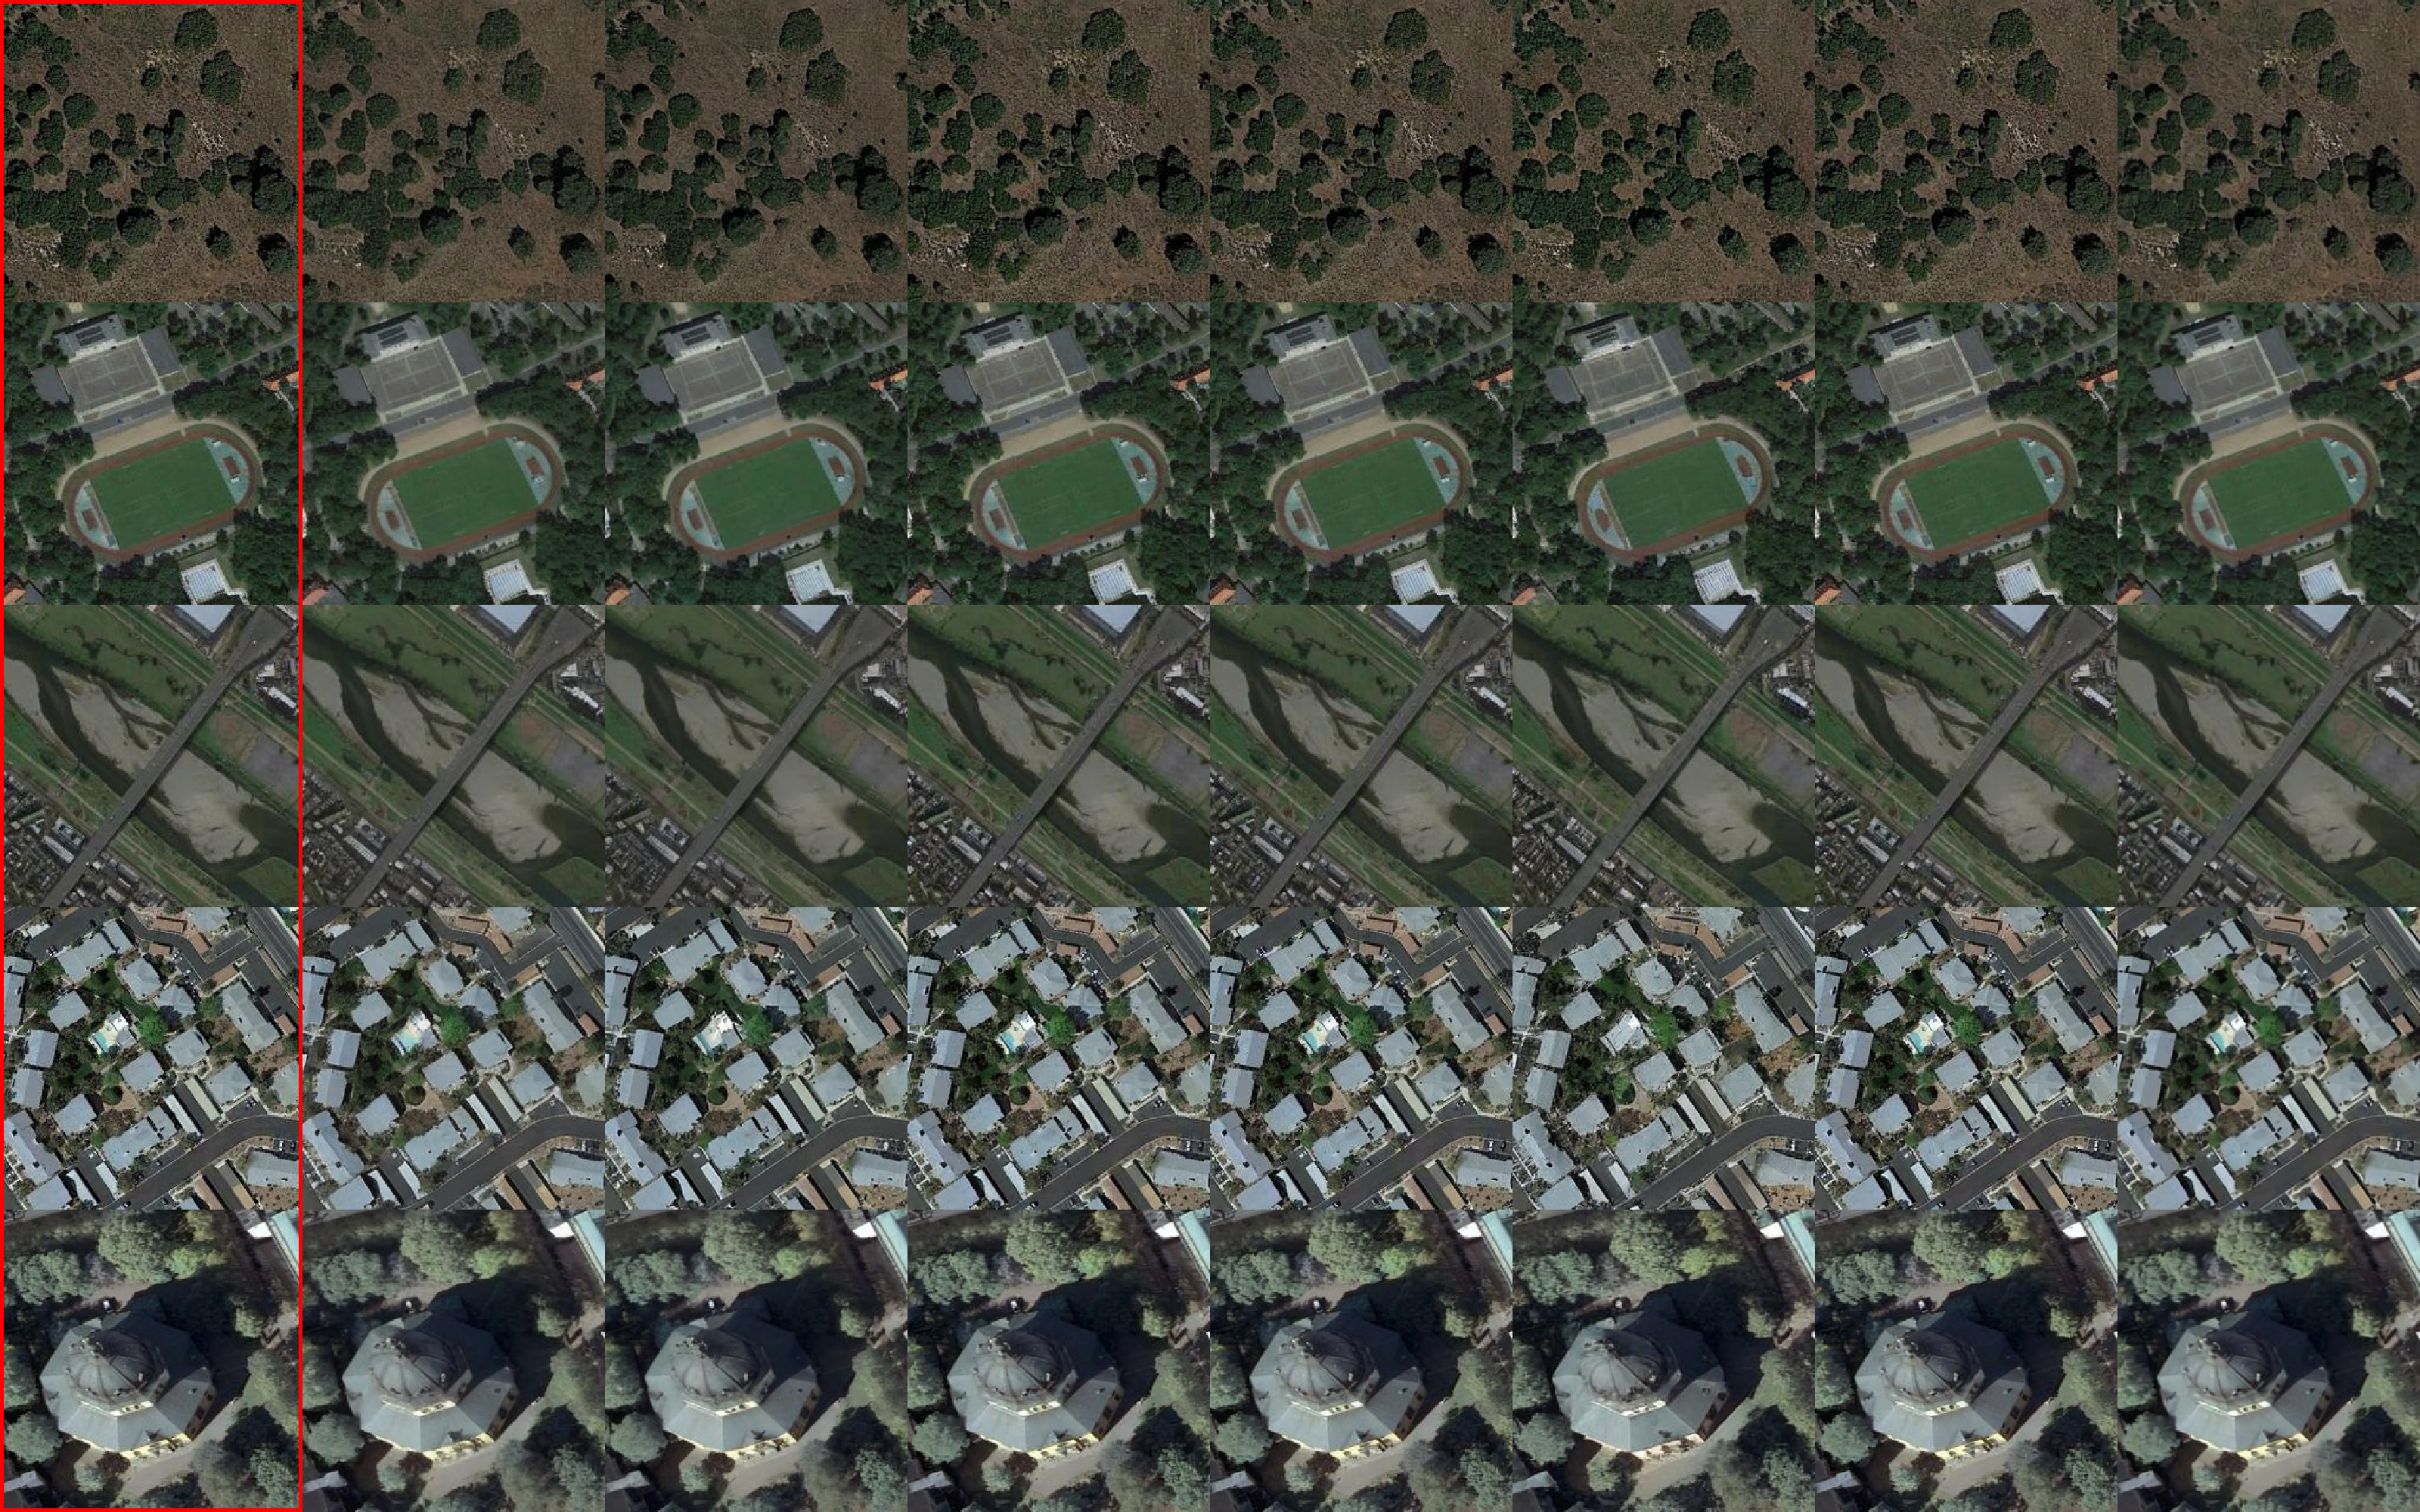
\includegraphics[width=1.0\textwidth]{figures/RESULT5samples.pdf}
\caption{Qualitative reconstructions from 5 random RESISC45 samples. Each column shows (left to right): Original, SD21-VAE, SDXL-VAE, SD35-VAE, FLUX1-VAE, SANA-VAE, FLUX2-VAE, and Qwen-VAE. No significant visual difference appears.}
\label{fig:reconstruction_examples}
\end{figure}

\section{Insights and Conclusion}

\textbf{Insights 1:} We find that VAEs reconstruct remote sensing images remarkably well, with reconstructions appearing visually nearly identical to the input. We argue that VAEs may have the potential to implicitly deblur and denoise input images, where the reconstructed image serves as a better data source for model training (e.g., representation learning) with possibly improved statistics.

\textbf{Insights 2:} As the compression appears effectively lossless, we argue for directly storing latent representations instead of original images as datasets to reduce storage requirements. 

In this work, we explored the robustness of natural image priors in VAEs for remote sensing. Our findings indicate that these models, when used zero-shot, can provide significant utility in data compression across various categories. We will release the reconstructed images along with their corresponding latents for community exploration and further research.


\bibliography{iclr2026_conference}
\bibliographystyle{iclr2026_conference}

% \newpage
% \appendix
% \section{Appendix}
% If you choose to include an appendix, please submit it as a separate PDF file.

\end{document}
